\chapter{WASM: verso il Web come piattaforma per la programmazione distribuita}
\label{chap:1}

\section{Contestualizzazione}
\label{sec:Contestualizzazione}

\subsection{Trend di evoluzione del Web}
Inizialmente le applicazioni Web erano costituite da semplici \textbf{pagine statiche} contenenti testo e immagini.
Con l'evoluzione dell'ecosistema Web, negli ultimi anni si è assistito a una trasformazione radicale delle applicazioni, guidata da una serie di tendenze e innovazioni tecnologiche che hanno portato a un'esperienza utente sempre più coinvolgente e interattiva.
\\L'introduzione di JavaScript e di librerie e framework correlati, hanno progressivamente arricchito l'interazione con le applicazioni Web, introducendo livelli crescenti di interattività e trasformando le semplici pagine statiche in ambienti dinamici e convolgenti. 
Un cambiamento significativo in tal senso, è avvenuto con l'avvento delle \textbf{Single Page Application (SPA)} e di \textbf{AJAX}.
Questo approccio ha rivoluzionato il tradizionale modello di navigazione e di sviluppo, consentendo alle applicazioni di essere caricate una sola volta e offrendo interazioni rapide e fluide grazie al caricamento dinamico di contenuti. Questo nuovo paradigma ha introdotto un'esperienza utente simile a quella delle applicazioni native, con transizioni scorrevoli tra le sezioni dell'applicazione e senza interruzioni visibili.
\\Parallelamente, la complessità delle funzionalità offerte è cresciuta in modo esponenziale, arrivando a ciò che viene riconosciuto come Web 3.0 o \textbf{Web Semantico}. Ormai è la norma spaziare da applicazioni che usano algoritmi di intelligenza artificiale, a simulatori, alla modifica istantanea di documenti, immagini e video.
\\Questo enorme sviluppo di funzionalità è stato trainato dalla crescente potenza di elaborazione dei dispositivi e dalla capacità delle tecnologie Web di sfruttare appieno queste risorse, facendo diventare normale interfacciarsi con siti Web in grado di gestire complesse operazioni in tempi rapidi.
\\Tuttavia questo progresso è stato accompagnato da un aumento smisurato del \textbf{numero di richieste} effettuate in rete e dall'utilizzo intensivo di risorse computazionali, sia lato cliente, che lato servitore.
È diventato cruciale bilanciare l'aggiunta di funzionalità sofisticate con la necessità di mantenere tempi di risposta rapidi e un'esperienza fluida per gli utenti. Inoltre, l'uso intensivo delle risorse ha sollevato questioni di scalabilità e di utilizzo efficiente delle risorse server.
\begin{figure}
        \begin{center}
                \includegraphics[width=0.9\columnwidth]{images/WebEvolution.png}
        \end{center}
        \caption{L'evoluzione del Web.}
        \label{fig:spa}
\end{figure}
        
\subsection{Importanza dell'ottimizzazione}
Ad oggi, l'ottimizzazione delle prestazioni è quindi diventata un aspetto cruciale nello sviluppo di applicazioni Web.
Gli utenti si aspettano interazioni con bassa latenza, caricamenti rapidi e risposte immediate.
Questa esigenza mette in risalto l'importanza di bilanciare l'aggiunta di nuove funzionalità, con l'offerta di una \emph{User Experience} ottimale.
\\I tempi di caricamento prolungati possono portare a un alto tasso di abbandono delle pagine, riducendo l'opportunità di coinvolgere nuovi utenti.
Inoltre, con l'aumentare dell'utilizzo di \textbf{dispositivi mobili} e di conseguenza, di \textbf{connessioni instabili}, l'ottimizzazione diventa ancor più critica per assicurare un'esperienza coerente su diverse piattaforme e condizioni di rete.
Tutto ciò non riguarda solo il lato client, ma coinvolge anche il lato server. 
Un carico eccessivo sui server può influire negativamente sulla scalabilità, causando ritardi nelle risposte e possibili interruzioni del servizio.
L'ottimizzazione deve quindi coinvolgere tutti gli aspetti dell'architettura delle applicazioni Web.
\\Nell'implementare ottimizzazioni, sono nati varie soluzioni interessanti. 
Ad esempio, per gestire task che svolgono molte operazioni di Input/Output si è distinto il runtime environment \textbf{Node.js}\cite*{nodeHome}, mentre per quanto riguardo l'esecuzione di attività che sfruttano molto la CPU è emerso \textbf{WebAssembly(Wasm)}\cite*{wasmHome}.
Quest'ultimo, nato inizialmente per consentire l'esecuzione di codice ad alta efficienza all'interno del browser, è diventato portabile anche su piattaforme server side grazie allo sviluppo dell'interfaccia di sistema \textbf{WebAssembly System Interface (WASI)}\cite*{wasiHome}.


\section{Motivazioni e Obiettivi}
\label{sec:Obiettivi}
La \textbf{crescente complessità} delle applicazioni Web e l'esigenza di offrire agli utenti esperienze interattive sempre più coinvolgenti hanno portato l'ambito dello sviluppo Web a una svolta significativa.
Le aspettative degli utenti si sono evolute verso applicazioni che offrano prestazioni reattive, interattività immediata e funzionalità avanzate.
\\È proprio questo insieme di aspettative a essere alla base delle motivazioni che hanno guidato la scelta del tema di questa tesi di laurea.
\\In particolare, la presente ricerca, si propone di confrontare in modo dettagliato, due differenti approcci di sviluppo per un'applicazione con funzionalità \textbf{fortemente CPU-intensive}.
\subsection{Tipologia di applicazione}
Per tale confronto, si è optato per una Web-app che implementi alcune tecniche di \textbf{elaborazione di immagini}.
In particolare, l'utente avrà la possibilità di eseguire l'upload di immagini su un server e indicare una serie di modifiche da apportare (ad esempio "ridimensionamento del 50\%"). Il server manipolerà i file in base ai parametri ricevuti e infine restituirà al cliente le immagini modificate.
\\Non verrà esplorato in modo approfondito il campo dell'elaborazione digitale di immagini, ma ci si limiterà all'implementazione di funzionalità usate spesso da utenti comuni, come ad esempio, ridimensionamento, rotazione, aumento/diminuzione di luminosità/contrasto e altre che verranno specificate nel capitolo \ref{chap:3}.
\\Tale tipologia di applicazione, si sposa bene per lo scopo finale della tesi: valutare come due approcci (e due linguaggi) piuttosto differenti, ma sempre più diffusi al giorno d'oggi, risolvano il problema di un'applicazione Web che svolga operazioni dall'alto costo computazionale.
\begin{figure}
        \begin{center}
                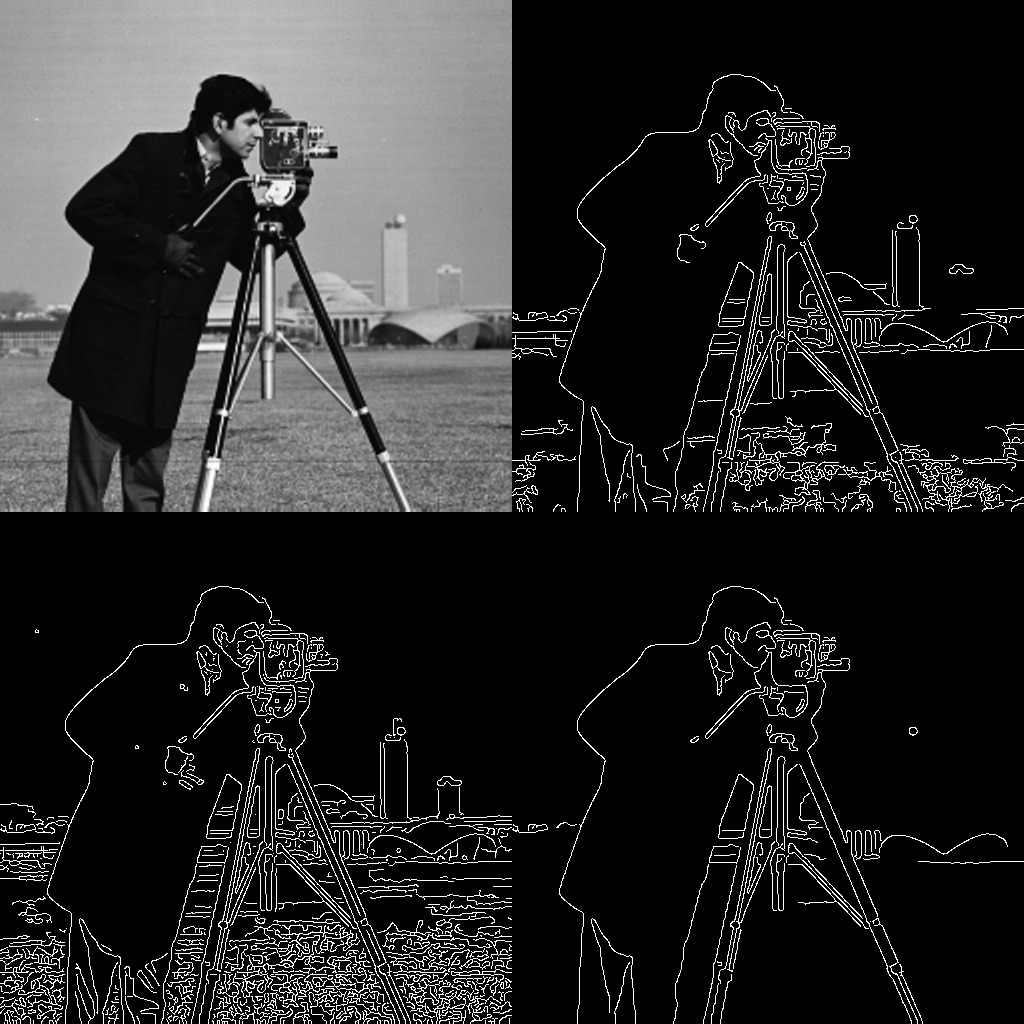
\includegraphics[width=0.55\columnwidth]{images/imageProc.jpg}
        \end{center}
        \caption[Image Processing]{Il campo dell'elaborazione digitale di immagini è molto ampio e sarebbe possibile integrare anche operazioni avanzate (edge detection, pattern recognition etc.), che richiederebbero risorse computazionali molto elevate. Per lo scopo di questa tesi ci si limiterà a elaborazioni più semplici, ma in ogni caso rilevanti e sufficienti a mettere alla prova la CPU.}
        \label{fig:imageProc}
\end{figure} 
\subsection{Metodologie confrontate}
Le due modalità di sviluppo in esame riguarderanno l'utilizzo delle tecnologie JavaScript e WebAssembly lato server e quindi rispettivamente del runtime environment Node.js e del linguaggio di programmazione \textbf{Rust} in combinazione con WebAssembly System Interface\cite*{rust:wasm}. 
\\La scelta di Node.js deriva dal suo utilizzo sempre maggiore grazie all'utilizzo del linguaggio JavaScript, dall'approccio asincrono nella gestione delle richieste e dalla sua ottima scalabilità per applicazioni fortemente File-System-Intensive.
Per quanto riguarda la seconda tecnologia si è invece optato per Rust, in quanto consente sia la scrittura di \textbf{moduli} successivamente \textbf{compilabili in WebAssembly}, sia il loro utilizzo efficiente all'interno del codice, mantenendo in questo modo un'ottima coerenza e risultando, teoricamente, una buona scelta per lo sviluppo di applicazioni computazionalmente complesse. 

\subsection{Analisi Comparativa delle Tecnologie}
Un elemento iniziale di questa ricerca sarà un'analisi dettagliata delle tecnologie prese in esame. 
Inizialmente, nel capitolo \ref{chap:2}, verrà svolta un'analisi comparativa delle due tecnologie, presentando i vantaggi e gli svantaggi teorici che caratterizzano entrambe le opzioni.
\\Sarà infatti fondamentale comprendere come ciascuna affronti la complessità legata ad operazioni I/O-intensive e CPU-intensive. Questo ci permetterà di valutare nel modo più opportuno i risultati che emergeranno succesivamente durante i test e i benchmark dell'applicazione sviluppata.
\begin{figure}
        \begin{center}
                
\includegraphics[width=0.4\columnwidth]{images/rustwasm.jpg}
        \end{center}
        \caption{Rust e WebAssembly}
        \label{fig:rustwasm}
\end{figure}
\newpage
Si procederà poi ad illustrare in modo approfondito il funzionamento delle API sfruttate. Verranno analizzate le peculiarità del linguaggio Rust che lo rendono adatto ad applicazioni ad alta intensità computazionale. Allo stesso modo ci si soffermerà sull'efficacia di WebAssembly nell'esecuzione di codice di basso livello con prestazioni paragonabili a quelle dei linguaggi nativi.
\\Nel contempo si analizzerà anche la metodologia basata su Node.js, concentrandosi sull'efficienza e la flessibilità che questo ambiente di esecuzione JavaScript può offrire in ambito Web.
\begin{figure}
        \begin{center}
                
\includegraphics[width=0.3\columnwidth]{images/node.png}
        \end{center}
        \caption{Node.js}
        \label{fig:nodejs}
\end{figure} 
\\Si proseguirà affrontando un'approfondimento sulle prestazioni di ciascuna tecnologia, evidenziando scenari in cui una risulti più vantaggiosa. Questo approfondimento sarà alla base delle successive valutazioni sulle prestazioni delle applicazioni sviluppate con i due metodi presi in esame.

\subsection{Valutazione dell'Impatto di Wasm}
WebAssembly, in particolare, è emerso come \textbf{un'innovazione} cruciale nel mondo dello sviluppo Web.
Consentendo l'esecuzione di codice a basso livello con prestazioni paragonabili a quelle dei linguaggi nativi, Wasm offre la possibilità di ottenere prestazioni elevate all'interno di un ambiente browser-based.
\\Parallelamente, WebAssembly System Interface (WASI) gioca un ruolo chiave nell'estendere il potenziale di WebAssembly. WASI fornisce un'interfaccia standardizzata per l'\textbf{accesso a risorse di sistema}, consentendo alle applicazioni di interagire con l'ambiente circostante in modo controllato e sicuro. Tale capacità è particolarmente rilevante nell'ambito delle applicazioni Web CPU-intensive, in quanto consente di accedere, in maniera efficiente, alle risorse necessarie per eseguire complesse operazioni di calcolo e manipolazione dei dati.
\\Sarà quindi fondamentale valutare e cercare di misurare l'impatto di WASI, sia per quanto riguarda le prestazioni sia per quanto riguarda lo sviluppo e l'integrazione dello stesso all'interno di un'applicazione Web.

\subsection{Obiettivi}
Si intende esplorare le opportunità offerte dalle tecnologie enunciate sopra, nell'ottica di un'ottimizzazione delle prestazioni.
In questo contesto l'obiettivo centrale è quello di comprendere i \textbf{benefici specifici} legati a ciascun approccio, individuando le circostanze in cui uno dei due possa risultare vantaggioso in termini di \textbf{efficienza computazionale} e reattività. 
Inoltre si intende sottolineare il fatto che le decisioni intraprese sin dalla fase di progettazione, possono avere un impatto significativo sulle prestazioni e sull'esperienza utente di un'applicazione.
\\Si vuole mettere in evidenza l'importanza di una valutazione attenta e accurata dell'architettura e delle esigenze dell'applicazione stessa.
Aspetto da affrontare attraverso un'analisi dettagliata che considera le funzionalità dell'applicazione e valuta se esse siano orientate al calcolo intensivo o ad un'ampia manipolazione del File System.
\\Per raggiungere in maniera \textbf{efficace e quantificabile} gli obiettivi, verrà fatta un'analisi approfondita delle performance e delle prestazioni delle due applicazioni sviluppate.
Questo consentirà di valutare in modo empirico e misurabile l'impatto di ciascuna tecnologia nel contesto di applicazioni CPU-intensive.
\\Sarà inoltre trattato anche il tema della \textbf{scalabilità}. Esso diventa di primaria importanza quando i volumi di traffico e i carichi di lavoro aumentano. Valutare come diverse tecnologie gestiscano richieste concorrenti è fondamentale per determinare quale sia più adatta alle esigenze di un progetto.
\\Infine si considererà anche la \textbf{facilità di sviluppo e l'espandibilità}. 
Questi temi avanzano spesso di pari passo ed è importante, in un ambiente Web in rapida evoluzione, che un progetto si adatti facilmente, sia all'aggiunta di nuovi requisiti e funzionalità, sia all'integrazione con altri sistemi e servizi. Tale flessibilità può infatti avere un impatto significativo sulla vita e sulla sostenibilità di un progetto.


\newpage

\section{Struttura della tesi}
\label{sec:struttura}
La tesi seguirà una struttura articolata in modo da affrontare in maniera approfondita gli aspetti chiave delle tecnologie e delle analisi proposte.
\\Nel Capitolo \ref{chap:2}, sarà presentata una panoramica esaustiva delle tecnologie coinvolte in questa ricerca. Questo capitolo fornirà un'analisi dettagliata di WebAssembly/WASI in combinazione con Rust e di Node.js, esaminandone le caratteristiche, i vantaggi e le \textbf{API} utili allo sviluppo dell'applicazione.
Verranno esplorati i contesti in cui ciascuna tecnologia si dimostra più adeguata, fornendo le basi per una comprensione approfondita delle successive misurazioni e valutazioni.
\\Nel Capitolo \ref{chap:3}, il focus sarà sul prototipo dell'applicazione sviluppata. Saranno illustrate le scelte progettuali, l'architettura complessiva e le funzionalità implementate.
Successivamente, verranno presentati i dettagli delle misurazioni condotte, insieme ai criteri di valutazione delle prestazioni delle tecnologie in esame. 
Saranno discussi i risultati ottenuti e i confronti tra le diverse implementazioni, evidenziando gli aspetti in cui ognuno degli approcci studiati, si distingue in termini di ottimizzazione delle prestazioni.
